\chapter{Adjunct Therapy for Airway Management}
\label{ch:adjunct}

Ventilation is rarely the only treatment. Bronchodilators, steroids, mucolytics, surfactant, inhaled nitric oxide, airway clearance and prone positioning change the mechanics and gas exchange the ventilator works against. The model represents each adjunct by its effect on the parameters of \crefrange{ch:ch06}{ch:ch09}, not by pharmacology. A therapy multiplies airway resistance, lung compliance, shunt, low-$\dot V/\dot Q$ fraction or alveolar dead space, and the patient's response then emerges from the same equations as every other change.

\section{Effect model}
\label{sec:adj-model}
Each therapy $d$ has a set of target factors $f_R$, $f_C$, $f_{sh}$ and $f_{vq}$ for resistance, compliance, shunt and low-$\dot V/\dot Q$ fraction. Anticholinesterases instead have factors $f_{\mathrm{mus}}$ and $f_{\mathrm{MEP}}$ for inspiratory and expiratory muscle strength. A phenotype effectiveness $\sigma\in[0,1]$ scales the factor:
\begin{equation}
f_{\mathrm{eff}}=1-(1-f)\,\sigma .
\label{eq:adj-eff}
\end{equation}
A bronchodilator with $f_R=0.65$ therefore lowers resistance by 35\% in asthma ($\sigma=1$) and by none in fibrosis ($\sigma=0$). The effectiveness comes from the disease class of the loaded phenotype (\cref{tab:adj-defs}).

\paragraph{Default timing.} The current modifier $m$ moves toward its target $m^*$ once per breath,
\begin{equation}
m_{k+1}=m_k+(m^*-m_k)\bigl(1-e^{-T_{\mathrm{br}}/\tau}\bigr),
\label{eq:adj-tau}
\end{equation}
where $T_{\mathrm{br}}$ is the breath period. Fast agents use $\tau=\SI{30}{\second}$: bronchodilators, steroids, racemic epinephrine, surfactant, nitric oxide, hypertonic saline and the mechanical treatments. Mucolytics and inhaled antibiotics use $\tau=\SI{60}{\second}$. These are compressed times, chosen so that a response is seen within a teaching session. Each drug can be given once and wears off after ten minutes. Mechanical treatments can be repeated with diminishing returns, because each session clears less secretion than the one before; secretions re-accumulate after ten minutes.

\paragraph{Physiological timing.} An option replaces \cref{eq:adj-tau} with a Bateman onset--offset curve in simulated minutes,
\begin{equation}
E(t)=\frac{e^{-t/t_e}-e^{-t/t_a}}{e^{-t_p/t_e}-e^{-t_p/t_a}},\qquad
t_p=\frac{t_a t_e\ln(t_e/t_a)}{t_e-t_a},
\label{eq:adj-pk}
\end{equation}
where $t$ is the time since the dose, $t_a$ the absorption (onset) constant, $t_e$ the elimination constant and $t_p$ the time of peak effect, at which $E=1$ (\cref{fig:adj-pk}). Repeated doses of one drug combine as $1-\prod(1-E_i)$, and the parameter multiplier is $\prod_d\bigl[1-(1-f_d)E_d\bigr]$. In COPD the salbutamol resistance factor is 0.86, not 0.65, reflecting the smaller reversibility of fixed obstruction~\citep{calverley2003}.

\begin{figure}[htbp]\centering
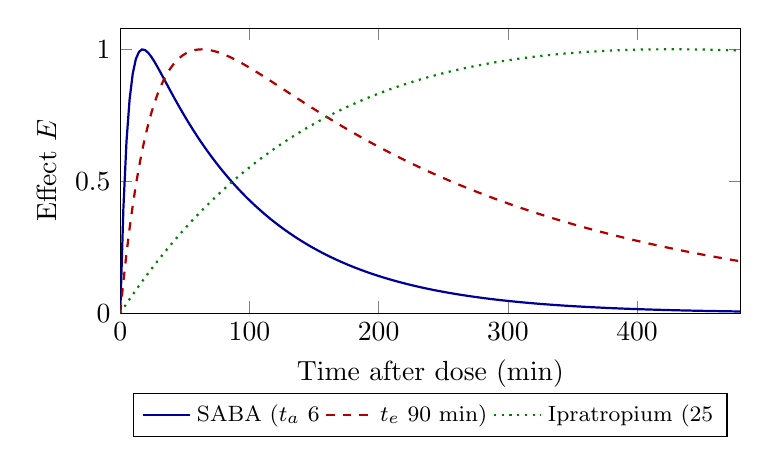
\begin{tikzpicture}
\begin{axis}[width=0.78\linewidth,height=5.2cm,xlabel={Time after dose (min)},ylabel={Effect $E$},xmin=0,xmax=480,ymin=0,ymax=1.08,legend style={font=\footnotesize,at={(0.5,-0.28)},anchor=north,legend columns=3},samples=200,domain=0.01:480]
\addplot[thick,blue!60!black]{(exp(-x/90)-exp(-x/6))/(exp(-17.37/90)-exp(-17.37/6))};
\addplot[thick,dashed,red!70!black]{(exp(-x/240)-exp(-x/25))/(exp(-63.2/240)-exp(-63.2/25))};
\addplot[thick,dotted,green!50!black]{(exp(-x/1440)-exp(-x/180))/(exp(-427.8/1440)-exp(-427.8/180))};
\legend{SABA ($t_a$ 6, $t_e$ 90 min),Ipratropium (25, 240),IV corticosteroid (180, 1440)}
\end{axis}
\end{tikzpicture}
\caption{Onset and offset curves of \cref{eq:adj-pk} for three adjuncts.}
\label{fig:adj-pk}
\end{figure}

\section{Therapy library}
\label{sec:adj-lib}

\begin{table}[htbp]\centering\scriptsize\setlength{\tabcolsep}{3pt}
\caption{Adjunct therapies as implemented. Factors multiply the parameter; 1 means no effect. $t_a$, $t_e$: onset and elimination constants of \cref{eq:adj-pk} (min). Full effectiveness $\sigma=1$ applies to the class shown; others receive the partial value listed or none.}
\label{tab:adj-defs}
\begin{tabular}{@{}>{\raggedright\arraybackslash}p{0.17\linewidth}cccccc>{\raggedright\arraybackslash}p{0.27\linewidth}l@{}}
\toprule
Therapy & $f_R$ & $f_C$ & $f_{sh}$ & $f_{vq}$ & $t_a$ & $t_e$ & Effectiveness & Source\\\midrule
SABA & 0.65 & 1 & 1 & 0.85 & 6 & 90 & obstructive; inflammatory 0.15 & --\\
LABA & 0.75 & 1 & 1 & 0.90 & 15 & 720 & obstructive & \citep{calverley2003}\\
Ipratropium & 0.82 & 1 & 1 & 0.92 & 25 & 240 & obstructive & \citep{rennard1996,gross1987}\\
MgSO\textsubscript{4} & 0.78 & 1 & 1 & 0.90 & 10 & 90 & asthma; other obstructive 0.3 & \citep{rowe2000}\\
IV corticosteroid & 0.90 & 1 & 0.92 & 0.88 & 180 & 1440 & obstructive or inflammatory & \citep{niewoehner1999}\\
Racemic epinephrine & 0.55 & 1 & 1 & 0.92 & 3 & 60 & croup, upper airway; obstructive 0.15 & \citep{westley1978}\\
Surfactant & 1 & 1.60 & 0.75 & 0.85 & 2 & 1440 & RDS, ARDS, MAS, CDH; atelectasis 0.4 & \citep{engle2008}\\
Inhaled NO & 1 & 1 & 0.72 & 0.82 & 1 & -- & PPHN, ARDS; inflammatory 0.3 & \citep{clark2000}\\
Hypertonic saline & 0.90 & 1 & 1 & 0.90 & 10 & 120 & CF, bronchiectasis; secretions 0.7 & \citep{donaldson2006}\\
N-acetylcysteine & 0.82 & 1 & 1 & 0.90 & 30 & 360 & CF, bronchiectasis; secretions 0.7; obstructive 0.4 & \citep{sheffner1963,decramer2005}\\
Dornase alfa & 0.72 & 1 & 1 & 0.85 & 60 & 720 & CF, bronchiectasis; secretions 0.3 & \citep{fuchs1994}\\
Inhaled antibiotics & 0.90 & 1 & 0.90 & 0.90 & 60 & 720 & CF, bronchiectasis; secretions 0.5 & \citep{ramsey1999}\\
HFCWO vest & 0.85 & 1 & 1 & 0.90 & -- & -- & secretions; NMD 0.5; others 0.2 & \citep{nicolini2013}\\
Insufflation--exsufflation & 0.80 & 1 & 0.95 & 0.88 & -- & -- & NMD; secretions 0.6; others 0.15 & \citep{bach1993}\\
Oral suction & 0.98 & 1 & 1 & 0.99 & -- & -- & secretions 0.8; NMD 0.6; others 0.3 & --\\
Tracheal suction & 0.80 & 1 & 0.96 & 0.92 & -- & -- & secretions 1; NMD 0.7; others 0.4 & --\\
Prone position & 1 & 1 & 0.72 & 0.78 & -- & -- & atelectatic or ARDS & \citep{guerin2013}\\\midrule
Neostigmine IV & \multicolumn{4}{c}{MIP $\times1.33$, MEP $\times1.235$} & 8 & 60 & myasthenia only & \citep{radwan1988}\\
Pyridostigmine & \multicolumn{4}{c}{MIP $\times1.18$} & 50 & 150 & myasthenia only & --\\
\bottomrule
\end{tabular}
\end{table}

\paragraph{Bronchodilators and steroids.} The $\beta_2$-agonist, anticholinergic and magnesium factors lower resistance and improve low-$\dot V/\dot Q$ matching. Bronchodilation in COPD can briefly worsen PaO\textsubscript{2} by releasing hypoxic vasoconstriction in poorly ventilated units~\citep{gross1987}; the model does not represent this, because its low-$\dot V/\dot Q$ factor only improves. Steroids act slowly ($t_a=\SI{3}{\hour}$) and partly on gas exchange, consistent with their role in exacerbations~\citep{niewoehner1999}.

\paragraph{Surfactant and nitric oxide.} Surfactant raises lung compliance by 60\% and recruits units, lowering shunt~\citep{engle2008}. Inhaled nitric oxide vasodilates ventilated units and so lowers both the intrapulmonary shunt and the low-$\dot V/\dot Q$ fraction~\citep{clark2000}. The model does not reduce the extrapulmonary shunt of PPHN directly; it acts through the intrapulmonary shunt term.

\paragraph{Secretion clearance.} Mucoactive drugs and mechanical clearance lower resistance by removing secretions. Their effectiveness is highest where secretions dominate, in CF, bronchiectasis and exacerbations~\citep{donaldson2006,fuchs1994,ramsey1999}. Mechanical insufflation--exsufflation is most effective in neuromuscular weakness, where cough is the failing mechanism~\citep{bach1993}.

\paragraph{Prone position.} Prone position lowers shunt by 28\% and the low-$\dot V/\dot Q$ fraction by 22\% in atelectatic and ARDS phenotypes~\citep{guerin2013}. It also changes the esophageal pressure offset of \cref{sec:mech-pes}.

\paragraph{Anticholinesterases.} In myasthenia, neostigmine raises MIP by 33\% and MEP by 24\% at about 30 minutes~\citep{radwan1988}. Pyridostigmine has a slower onset and a smaller effect. These are the only adjuncts that act on the muscles of \cref{ch:ch07} rather than the lung.

\section{Limitations}
Effects are fixed fractions of the current parameter, not dose--response curves. They do not depend on drug dose, delivery route or the patient's ventilation, so a nebulized drug reaches the lungs equally in any mode. Effectiveness is assigned by disease class and does not vary between patients. Tolerance, side effects such as tachycardia, and drug interactions are not represented. The default timing is compressed for teaching, so only the physiological-timing option should be used for time courses.
